\documentclass[]{article}
\usepackage{lmodern}
\usepackage{amssymb,amsmath}
\usepackage{ifxetex,ifluatex}
\usepackage{fixltx2e} % provides \textsubscript
\ifnum 0\ifxetex 1\fi\ifluatex 1\fi=0 % if pdftex
  \usepackage[T1]{fontenc}
  \usepackage[utf8]{inputenc}
\else % if luatex or xelatex
  \ifxetex
    \usepackage{mathspec}
  \else
    \usepackage{fontspec}
  \fi
  \defaultfontfeatures{Ligatures=TeX,Scale=MatchLowercase}
\fi
% use upquote if available, for straight quotes in verbatim environments
\IfFileExists{upquote.sty}{\usepackage{upquote}}{}
% use microtype if available
\IfFileExists{microtype.sty}{%
\usepackage[]{microtype}
\UseMicrotypeSet[protrusion]{basicmath} % disable protrusion for tt fonts
}{}
\PassOptionsToPackage{hyphens}{url} % url is loaded by hyperref
\usepackage[unicode=true]{hyperref}
\hypersetup{
            pdftitle={econAssignments},
            pdfauthor={Jasmine Cui},
            pdfborder={0 0 0},
            breaklinks=true}
\urlstyle{same}  % don't use monospace font for urls
\usepackage[margin=1in]{geometry}
\usepackage{color}
\usepackage{fancyvrb}
\newcommand{\VerbBar}{|}
\newcommand{\VERB}{\Verb[commandchars=\\\{\}]}
\DefineVerbatimEnvironment{Highlighting}{Verbatim}{commandchars=\\\{\}}
% Add ',fontsize=\small' for more characters per line
\usepackage{framed}
\definecolor{shadecolor}{RGB}{248,248,248}
\newenvironment{Shaded}{\begin{snugshade}}{\end{snugshade}}
\newcommand{\KeywordTok}[1]{\textcolor[rgb]{0.13,0.29,0.53}{\textbf{#1}}}
\newcommand{\DataTypeTok}[1]{\textcolor[rgb]{0.13,0.29,0.53}{#1}}
\newcommand{\DecValTok}[1]{\textcolor[rgb]{0.00,0.00,0.81}{#1}}
\newcommand{\BaseNTok}[1]{\textcolor[rgb]{0.00,0.00,0.81}{#1}}
\newcommand{\FloatTok}[1]{\textcolor[rgb]{0.00,0.00,0.81}{#1}}
\newcommand{\ConstantTok}[1]{\textcolor[rgb]{0.00,0.00,0.00}{#1}}
\newcommand{\CharTok}[1]{\textcolor[rgb]{0.31,0.60,0.02}{#1}}
\newcommand{\SpecialCharTok}[1]{\textcolor[rgb]{0.00,0.00,0.00}{#1}}
\newcommand{\StringTok}[1]{\textcolor[rgb]{0.31,0.60,0.02}{#1}}
\newcommand{\VerbatimStringTok}[1]{\textcolor[rgb]{0.31,0.60,0.02}{#1}}
\newcommand{\SpecialStringTok}[1]{\textcolor[rgb]{0.31,0.60,0.02}{#1}}
\newcommand{\ImportTok}[1]{#1}
\newcommand{\CommentTok}[1]{\textcolor[rgb]{0.56,0.35,0.01}{\textit{#1}}}
\newcommand{\DocumentationTok}[1]{\textcolor[rgb]{0.56,0.35,0.01}{\textbf{\textit{#1}}}}
\newcommand{\AnnotationTok}[1]{\textcolor[rgb]{0.56,0.35,0.01}{\textbf{\textit{#1}}}}
\newcommand{\CommentVarTok}[1]{\textcolor[rgb]{0.56,0.35,0.01}{\textbf{\textit{#1}}}}
\newcommand{\OtherTok}[1]{\textcolor[rgb]{0.56,0.35,0.01}{#1}}
\newcommand{\FunctionTok}[1]{\textcolor[rgb]{0.00,0.00,0.00}{#1}}
\newcommand{\VariableTok}[1]{\textcolor[rgb]{0.00,0.00,0.00}{#1}}
\newcommand{\ControlFlowTok}[1]{\textcolor[rgb]{0.13,0.29,0.53}{\textbf{#1}}}
\newcommand{\OperatorTok}[1]{\textcolor[rgb]{0.81,0.36,0.00}{\textbf{#1}}}
\newcommand{\BuiltInTok}[1]{#1}
\newcommand{\ExtensionTok}[1]{#1}
\newcommand{\PreprocessorTok}[1]{\textcolor[rgb]{0.56,0.35,0.01}{\textit{#1}}}
\newcommand{\AttributeTok}[1]{\textcolor[rgb]{0.77,0.63,0.00}{#1}}
\newcommand{\RegionMarkerTok}[1]{#1}
\newcommand{\InformationTok}[1]{\textcolor[rgb]{0.56,0.35,0.01}{\textbf{\textit{#1}}}}
\newcommand{\WarningTok}[1]{\textcolor[rgb]{0.56,0.35,0.01}{\textbf{\textit{#1}}}}
\newcommand{\AlertTok}[1]{\textcolor[rgb]{0.94,0.16,0.16}{#1}}
\newcommand{\ErrorTok}[1]{\textcolor[rgb]{0.64,0.00,0.00}{\textbf{#1}}}
\newcommand{\NormalTok}[1]{#1}
\usepackage{graphicx,grffile}
\makeatletter
\def\maxwidth{\ifdim\Gin@nat@width>\linewidth\linewidth\else\Gin@nat@width\fi}
\def\maxheight{\ifdim\Gin@nat@height>\textheight\textheight\else\Gin@nat@height\fi}
\makeatother
% Scale images if necessary, so that they will not overflow the page
% margins by default, and it is still possible to overwrite the defaults
% using explicit options in \includegraphics[width, height, ...]{}
\setkeys{Gin}{width=\maxwidth,height=\maxheight,keepaspectratio}
\IfFileExists{parskip.sty}{%
\usepackage{parskip}
}{% else
\setlength{\parindent}{0pt}
\setlength{\parskip}{6pt plus 2pt minus 1pt}
}
\setlength{\emergencystretch}{3em}  % prevent overfull lines
\providecommand{\tightlist}{%
  \setlength{\itemsep}{0pt}\setlength{\parskip}{0pt}}
\setcounter{secnumdepth}{0}
% Redefines (sub)paragraphs to behave more like sections
\ifx\paragraph\undefined\else
\let\oldparagraph\paragraph
\renewcommand{\paragraph}[1]{\oldparagraph{#1}\mbox{}}
\fi
\ifx\subparagraph\undefined\else
\let\oldsubparagraph\subparagraph
\renewcommand{\subparagraph}[1]{\oldsubparagraph{#1}\mbox{}}
\fi

% set default figure placement to htbp
\makeatletter
\def\fps@figure{htbp}
\makeatother


\title{econAssignments}
\author{Jasmine Cui}
\date{1/21/2020}

\begin{document}
\maketitle

\section{Assignment 1}\label{assignment-1}

\subsection{Part I}\label{part-i}

\begin{Shaded}
\begin{Highlighting}[]
\NormalTok{myDog <-}\StringTok{ "Caramel"}
\KeywordTok{save}\NormalTok{(myDog, }\DataTypeTok{file =} \StringTok{'econAssi1+2.Rda'}\NormalTok{)}
\KeywordTok{load}\NormalTok{(}\StringTok{'econAssi1+2.Rda'}\NormalTok{)}
\end{Highlighting}
\end{Shaded}

\begin{Shaded}
\begin{Highlighting}[]
\CommentTok{# Header}
\CommentTok{# Use the library function to library tidyverse which will also contain ggplot and dplyr}
\KeywordTok{library}\NormalTok{(tidyverse)}
\end{Highlighting}
\end{Shaded}

\begin{verbatim}
## -- Attaching packages ------------------------------------------------------ tidyverse 1.3.0 --
\end{verbatim}

\begin{verbatim}
## v ggplot2 3.2.1     v purrr   0.3.3
## v tibble  2.1.3     v dplyr   0.8.3
## v tidyr   1.0.0     v stringr 1.4.0
## v readr   1.3.1     v forcats 0.4.0
\end{verbatim}

\begin{verbatim}
## -- Conflicts --------------------------------------------------------- tidyverse_conflicts() --
## x dplyr::filter() masks stats::filter()
## x dplyr::lag()    masks stats::lag()
\end{verbatim}

\begin{Shaded}
\begin{Highlighting}[]
\CommentTok{# Clear away the environment :-)}
\KeywordTok{rm}\NormalTok{(}\DataTypeTok{list =} \KeywordTok{ls}\NormalTok{())}

\CommentTok{# Set the working directory! }
\KeywordTok{setwd}\NormalTok{(}\StringTok{'/Users/jasminecui/Desktop/Metrics'}\NormalTok{)}

\CommentTok{# Create the object "birthday"}
\NormalTok{birthday <-}\StringTok{ }\DecValTok{04171999}

\KeywordTok{set.seed}\NormalTok{(birthday)}

\CommentTok{#    '}
\CommentTok{#    /}
\CommentTok{#    //                   .`"`.}
\CommentTok{#    ((___________________/() d `--,}
\CommentTok{#    | D O G of G E N E I T Y  -._./}
\CommentTok{#   |     _____________   /```^^`}
\CommentTok{#    --   |             |||}
\CommentTok{#    || /              |||}
\CommentTok{#    || |              |||}
\CommentTok{#    <<...>            <<.>}
\end{Highlighting}
\end{Shaded}

\subsection{Part II}\label{part-ii}

\begin{Shaded}
\begin{Highlighting}[]
\CommentTok{# (1)}
\CommentTok{# Flip a coin 10 times and generate mean; repeat process 1000 times }
\NormalTok{sampleMeans <-}\StringTok{ }\KeywordTok{vector}\NormalTok{() }
\ControlFlowTok{for}\NormalTok{ (i }\ControlFlowTok{in} \DecValTok{1}\OperatorTok{:}\DecValTok{1000}\NormalTok{) \{}
\NormalTok{  sampleMeans[i] <-}\StringTok{ }\KeywordTok{mean}\NormalTok{(}\KeywordTok{sample}\NormalTok{(}\DecValTok{0}\OperatorTok{:}\DecValTok{1}\NormalTok{, }\DecValTok{10}\NormalTok{, }\DataTypeTok{replace =} \OtherTok{TRUE}\NormalTok{))}
\NormalTok{\}}

\CommentTok{# Plot the distribution of the means gathered above }
\KeywordTok{hist}\NormalTok{(sampleMeans)}
\end{Highlighting}
\end{Shaded}

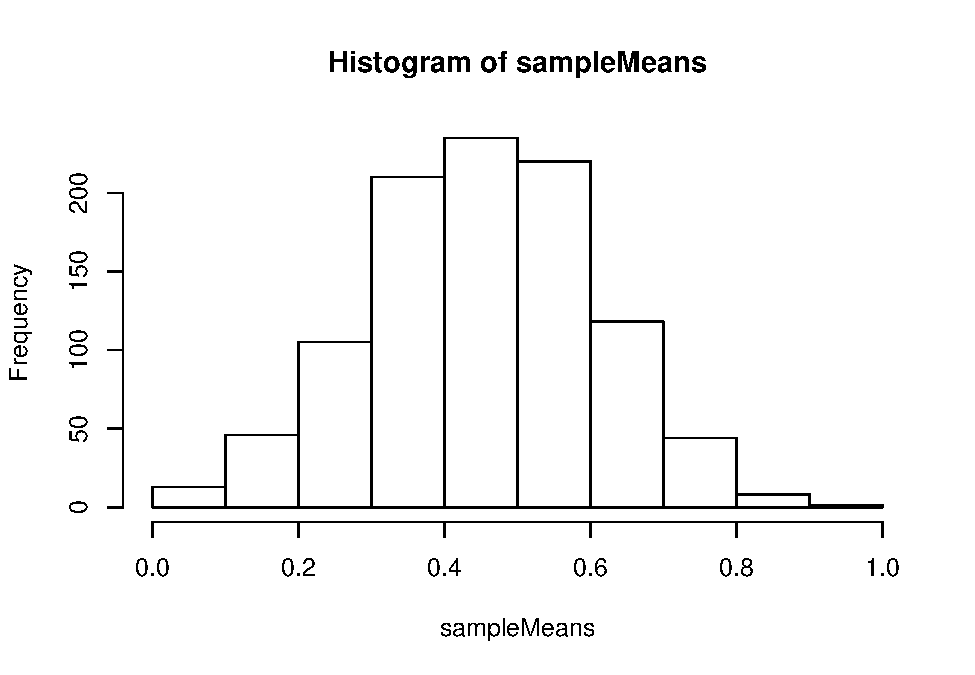
\includegraphics{macroNoGiodP_files/figure-latex/unnamed-chunk-2-1.pdf}

\begin{Shaded}
\begin{Highlighting}[]
\CommentTok{# Find the mean of the sample means }
\KeywordTok{summary}\NormalTok{(sampleMeans)}
\end{Highlighting}
\end{Shaded}

\begin{verbatim}
##    Min. 1st Qu.  Median    Mean 3rd Qu.    Max. 
##  0.0000  0.4000  0.5000  0.5014  0.6000  1.0000
\end{verbatim}

\begin{Shaded}
\begin{Highlighting}[]
\CommentTok{# The mean of the means is 0.4858}

\CommentTok{# Find the standard deviation of the sample means }
\KeywordTok{sd}\NormalTok{(sampleMeans)}
\end{Highlighting}
\end{Shaded}

\begin{verbatim}
## [1] 0.1582501
\end{verbatim}

\begin{Shaded}
\begin{Highlighting}[]
\CommentTok{# The SD of the sample means is 0.16}

\CommentTok{# (2)}
\CommentTok{# Flip a coin 100 times and generate mean; repeat process 1000 times}
\NormalTok{sampleMeans2 <-}\StringTok{ }\KeywordTok{vector}\NormalTok{()}
\ControlFlowTok{for}\NormalTok{ (i }\ControlFlowTok{in} \DecValTok{1}\OperatorTok{:}\DecValTok{1000}\NormalTok{) \{ }
\NormalTok{  sampleMeans2[i] <-}\StringTok{ }\KeywordTok{mean}\NormalTok{(}\KeywordTok{sample}\NormalTok{(}\DecValTok{0}\OperatorTok{:}\DecValTok{1}\NormalTok{, }\DecValTok{100}\NormalTok{, }\DataTypeTok{replace =} \OtherTok{TRUE}\NormalTok{))}
\NormalTok{\}}

\CommentTok{# Plot the distribution of the means gathered above}
\KeywordTok{hist}\NormalTok{(sampleMeans2)}
\end{Highlighting}
\end{Shaded}

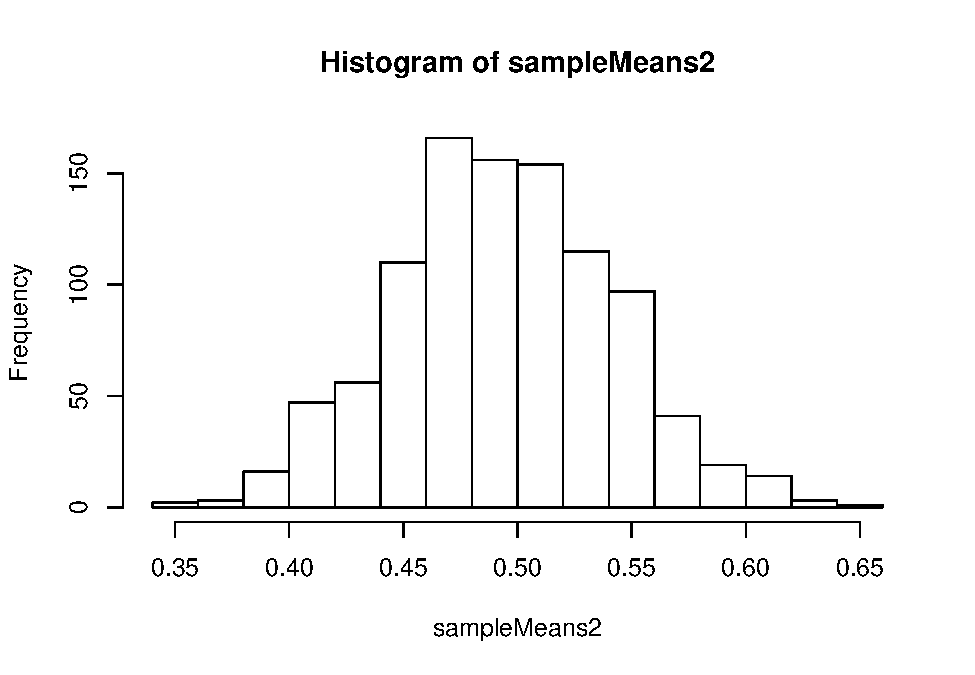
\includegraphics{macroNoGiodP_files/figure-latex/unnamed-chunk-2-2.pdf}

\begin{Shaded}
\begin{Highlighting}[]
\CommentTok{# Find the mean of the sample means }
\KeywordTok{summary}\NormalTok{(sampleMeans2)}
\end{Highlighting}
\end{Shaded}

\begin{verbatim}
##    Min. 1st Qu.  Median    Mean 3rd Qu.    Max. 
##  0.3500  0.4700  0.5000  0.4989  0.5300  0.6500
\end{verbatim}

\begin{Shaded}
\begin{Highlighting}[]
\CommentTok{# The mean of the means is 0.4972}

\CommentTok{# Find the standard deviation of the sample means }
\KeywordTok{sd}\NormalTok{(sampleMeans2)}
\end{Highlighting}
\end{Shaded}

\begin{verbatim}
## [1] 0.04760346
\end{verbatim}

\begin{Shaded}
\begin{Highlighting}[]
\CommentTok{# The SD of the sample means s 0.05}
\end{Highlighting}
\end{Shaded}

\section{Assignment 2}\label{assignment-2}

\subsection{Part I}\label{part-i-1}

\begin{Shaded}
\begin{Highlighting}[]
\CommentTok{# Perform a data generating process }

\NormalTok{population <-}\StringTok{ }\KeywordTok{vector}\NormalTok{()}
\ControlFlowTok{for}\NormalTok{ (i }\ControlFlowTok{in} \DecValTok{1}\OperatorTok{:}\DecValTok{1000000}\NormalTok{) \{}
\NormalTok{  x =}\StringTok{ }\KeywordTok{rnorm}\NormalTok{(}\DecValTok{1}\NormalTok{, }\DataTypeTok{mean =} \DecValTok{10}\NormalTok{, }\DataTypeTok{sd =} \DecValTok{2}\NormalTok{)}
\NormalTok{  u =}\StringTok{ }\KeywordTok{rnorm}\NormalTok{(}\DecValTok{1}\NormalTok{, }\DataTypeTok{mean =} \DecValTok{0}\NormalTok{, }\DataTypeTok{sd =} \DecValTok{3}\NormalTok{)}
\NormalTok{  population[i] <-}\StringTok{ }\DecValTok{8} \OperatorTok{+}\StringTok{ }\DecValTok{4}\OperatorTok{*}\NormalTok{x }\OperatorTok{+}\StringTok{ }\NormalTok{u }
\NormalTok{\}}
\end{Highlighting}
\end{Shaded}

\subsection{Part II}\label{part-ii-1}

\begin{Shaded}
\begin{Highlighting}[]
\NormalTok{x <-}\StringTok{ }\KeywordTok{c}\NormalTok{(}\DecValTok{1}\NormalTok{, }\DecValTok{2}\NormalTok{, }\DecValTok{3}\NormalTok{, }\DecValTok{4}\NormalTok{, }\DecValTok{5}\NormalTok{, }\DecValTok{6}\NormalTok{, }\DecValTok{7}\NormalTok{, }\DecValTok{8}\NormalTok{, }\DecValTok{9}\NormalTok{, }\DecValTok{10}\NormalTok{)}
\NormalTok{y <-}\StringTok{ }\KeywordTok{c}\NormalTok{(}\DecValTok{5}\NormalTok{, }\DecValTok{7}\NormalTok{, }\DecValTok{8}\NormalTok{, }\DecValTok{8}\NormalTok{, }\DecValTok{10}\NormalTok{, }\DecValTok{12}\NormalTok{, }\DecValTok{11}\NormalTok{, }\DecValTok{15}\NormalTok{, }\DecValTok{19}\NormalTok{, }\DecValTok{18}\NormalTok{)}
\NormalTok{j <-}\StringTok{ }\KeywordTok{c}\NormalTok{(}\DecValTok{7}\NormalTok{, }\DecValTok{7}\NormalTok{, }\DecValTok{7}\NormalTok{, }\DecValTok{8}\NormalTok{, }\DecValTok{8}\NormalTok{, }\DecValTok{7}\NormalTok{, }\DecValTok{8}\NormalTok{, }\DecValTok{8}\NormalTok{, }\DecValTok{7}\NormalTok{, }\DecValTok{6}\NormalTok{, }\DecValTok{9}\NormalTok{, }\DecValTok{9}\NormalTok{, }\DecValTok{8}\NormalTok{, }\DecValTok{9}\NormalTok{, }\DecValTok{7}\NormalTok{, }\DecValTok{8}\NormalTok{, }\DecValTok{9}\NormalTok{, }\DecValTok{6}\NormalTok{, }\DecValTok{10}\NormalTok{, }\DecValTok{10}\NormalTok{, }\DecValTok{9}\NormalTok{)}
\NormalTok{k <-}\StringTok{ }\KeywordTok{c}\NormalTok{(}\DecValTok{18}\NormalTok{, }\DecValTok{16}\NormalTok{, }\DecValTok{15}\NormalTok{, }\DecValTok{16}\NormalTok{, }\DecValTok{10}\NormalTok{, }\DecValTok{11}\NormalTok{, }\DecValTok{11}\NormalTok{, }\DecValTok{9}\NormalTok{, }\DecValTok{11}\NormalTok{, }\DecValTok{19}\NormalTok{, }\DecValTok{8}\NormalTok{, }\DecValTok{8}\NormalTok{, }\DecValTok{6}\NormalTok{, }\DecValTok{4}\NormalTok{, }\DecValTok{9}\NormalTok{, }\DecValTok{10}\NormalTok{, }\DecValTok{7}\NormalTok{, }\DecValTok{15}\NormalTok{, }\DecValTok{10}\NormalTok{, }\DecValTok{7}\NormalTok{, }\DecValTok{5}\NormalTok{)}

\CommentTok{# Does X or J look like it would have a greater variance? }
\CommentTok{# X looks like, immediately, like it would have a greater variance. This is because variance is a measure of variability and there is a lot more variability in X's observations than in J. If you look at the formula for calculating sample variance, you see that in the numerator it is the sum of the observed values minus the sample mean squared. Clearly, in X, a large number of the values are likely going to be further away from the sample mean than in J, where the values are pretty much clustered tightly around the mean. }
\CommentTok{# a. Find the sample variance of x and y}

\CommentTok{# Find the sample variance of x using the var() function}
\KeywordTok{var}\NormalTok{(x)}
\end{Highlighting}
\end{Shaded}

\begin{verbatim}
## [1] 9.166667
\end{verbatim}

\begin{Shaded}
\begin{Highlighting}[]
\CommentTok{# The sample variance is 9.17}

\CommentTok{# Find the sample variance of y using the var() function}
\KeywordTok{var}\NormalTok{(y)}
\end{Highlighting}
\end{Shaded}

\begin{verbatim}
## [1] 22.23333
\end{verbatim}

\begin{Shaded}
\begin{Highlighting}[]
\CommentTok{# The sample variance is 22.23}

\CommentTok{# b. Find the sample covariance of x and y}
\KeywordTok{cov}\NormalTok{(x,y)}
\end{Highlighting}
\end{Shaded}

\begin{verbatim}
## [1] 13.72222
\end{verbatim}

\begin{Shaded}
\begin{Highlighting}[]
\CommentTok{# The covariance of x and y is 13.72}

\CommentTok{# c. Find the sample variance of j and k}

\CommentTok{# Find the sample variance of j using the var() function}
\KeywordTok{var}\NormalTok{(j)}
\end{Highlighting}
\end{Shaded}

\begin{verbatim}
## [1] 1.347619
\end{verbatim}

\begin{Shaded}
\begin{Highlighting}[]
\CommentTok{# The sample variance is 1.35}

\CommentTok{# Find the sample variance of k using the var() function}
\KeywordTok{var}\NormalTok{(k)}
\end{Highlighting}
\end{Shaded}

\begin{verbatim}
## [1] 18.21429
\end{verbatim}

\begin{Shaded}
\begin{Highlighting}[]
\CommentTok{# The sample variance is 18.21}

\CommentTok{# d. Find the sample covariance of j and k}
\KeywordTok{cov}\NormalTok{(j,k)}
\end{Highlighting}
\end{Shaded}

\begin{verbatim}
## [1] -3.564286
\end{verbatim}

\begin{Shaded}
\begin{Highlighting}[]
\CommentTok{# The covariance of j and k is -3.56}

\CommentTok{# Present scatterplots of \{x, y\} and \{j, k\}}

\CommentTok{# Plot \{x, y\} using the plot() function}
\KeywordTok{plot}\NormalTok{(x, y)}
\end{Highlighting}
\end{Shaded}

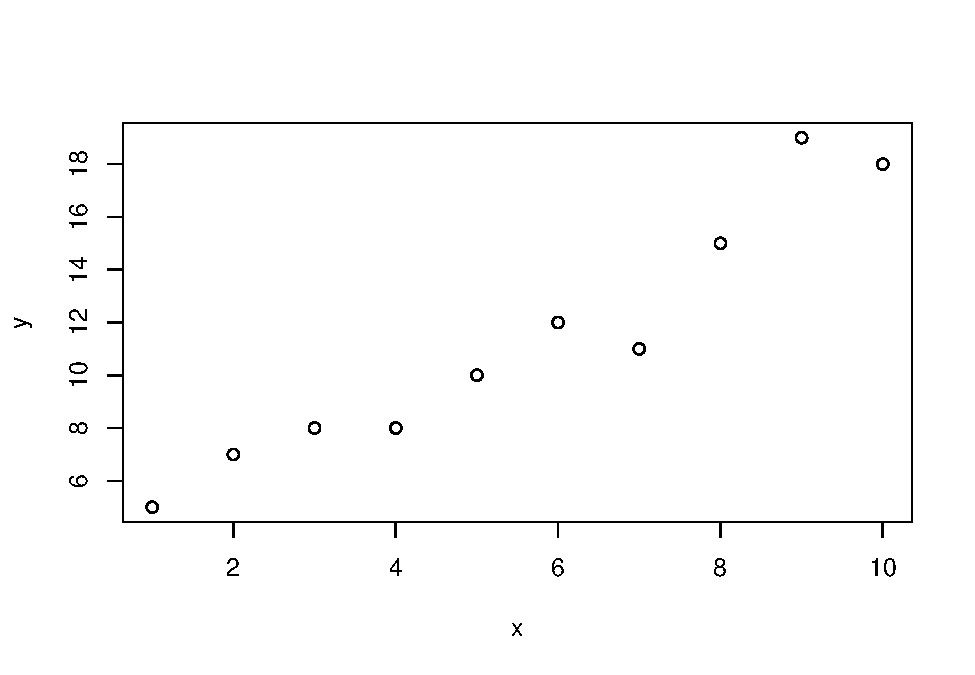
\includegraphics{macroNoGiodP_files/figure-latex/unnamed-chunk-4-1.pdf}

\begin{Shaded}
\begin{Highlighting}[]
\CommentTok{# Plot \{j, k\} using the plot() function}
\KeywordTok{plot}\NormalTok{(j, k)}
\end{Highlighting}
\end{Shaded}

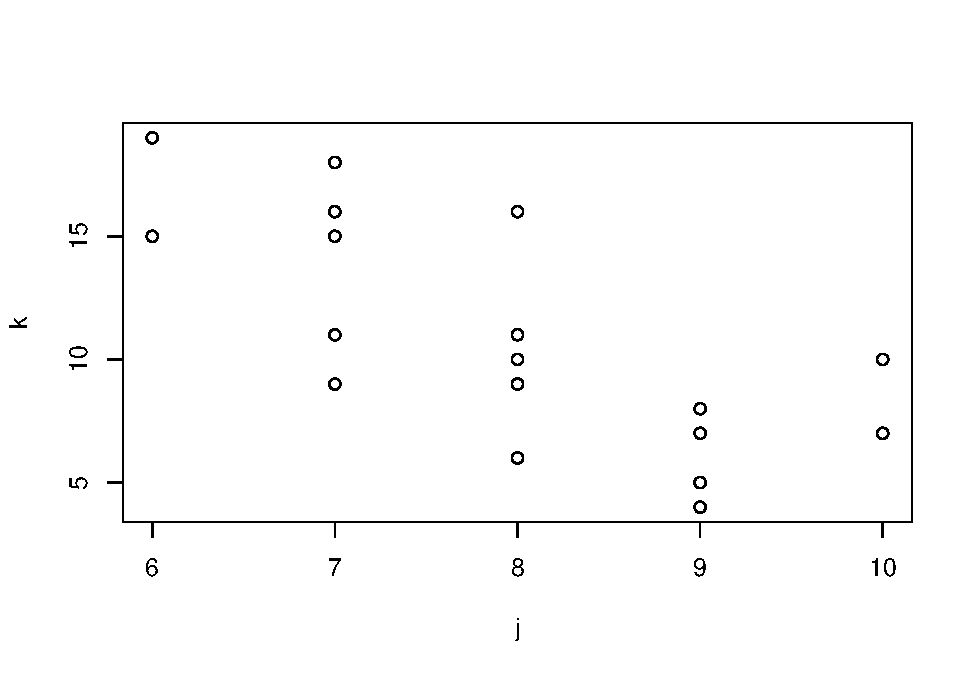
\includegraphics{macroNoGiodP_files/figure-latex/unnamed-chunk-4-2.pdf}

\section{Assignment 3}\label{assignment-3}

\subsection{Part I}\label{part-i-2}

\begin{Shaded}
\begin{Highlighting}[]
\CommentTok{# Take a sample of 1000 observations from the population data}
\NormalTok{ypop <-}\StringTok{ }\KeywordTok{vector}\NormalTok{()}
\NormalTok{xpop <-}\StringTok{ }\KeywordTok{vector}\NormalTok{()}
\ControlFlowTok{for}\NormalTok{ (i }\ControlFlowTok{in} \DecValTok{1}\OperatorTok{:}\DecValTok{1000}\NormalTok{) \{}
\NormalTok{  x =}\StringTok{ }\KeywordTok{rnorm}\NormalTok{(}\DecValTok{1}\NormalTok{, }\DataTypeTok{mean =} \DecValTok{10}\NormalTok{, }\DataTypeTok{sd =} \DecValTok{2}\NormalTok{)}
\NormalTok{  u =}\StringTok{ }\KeywordTok{rnorm}\NormalTok{(}\DecValTok{1}\NormalTok{, }\DataTypeTok{mean =} \DecValTok{0}\NormalTok{, }\DataTypeTok{sd =} \DecValTok{3}\NormalTok{)}
\NormalTok{  ypop[i] <-}\StringTok{ }\DecValTok{8} \OperatorTok{+}\StringTok{ }\DecValTok{4}\OperatorTok{*}\NormalTok{x }\OperatorTok{+}\StringTok{ }\NormalTok{u }
\NormalTok{  xpop[i] <-}\StringTok{ }\NormalTok{x}
\NormalTok{\}}

\CommentTok{# Manually calculate beta0hat and beta1hat using the sum() and var() functions }

\CommentTok{# Calculate beta1hat first using the formula cov(x, y) / var(x)}
\NormalTok{beta1hat <-}\StringTok{ }\KeywordTok{cov}\NormalTok{(xpop, ypop) }\OperatorTok{/}\StringTok{ }\KeywordTok{var}\NormalTok{(xpop)}
\CommentTok{# beta 1 is 4.01}

\CommentTok{# Calculate beta0hat using the equation y bar minus beta 1 hat multiplied by x bar }
\NormalTok{beta0hat <-}\StringTok{ }\KeywordTok{mean}\NormalTok{(ypop) }\OperatorTok{-}\StringTok{ }\NormalTok{beta1hat}\OperatorTok{*}\KeywordTok{mean}\NormalTok{(xpop)}
\CommentTok{# beta 0 is 7.89}

\CommentTok{# Check if these values look reasonable by creating a plot using the plot() function}
\KeywordTok{plot}\NormalTok{(xpop, ypop)}
\end{Highlighting}
\end{Shaded}

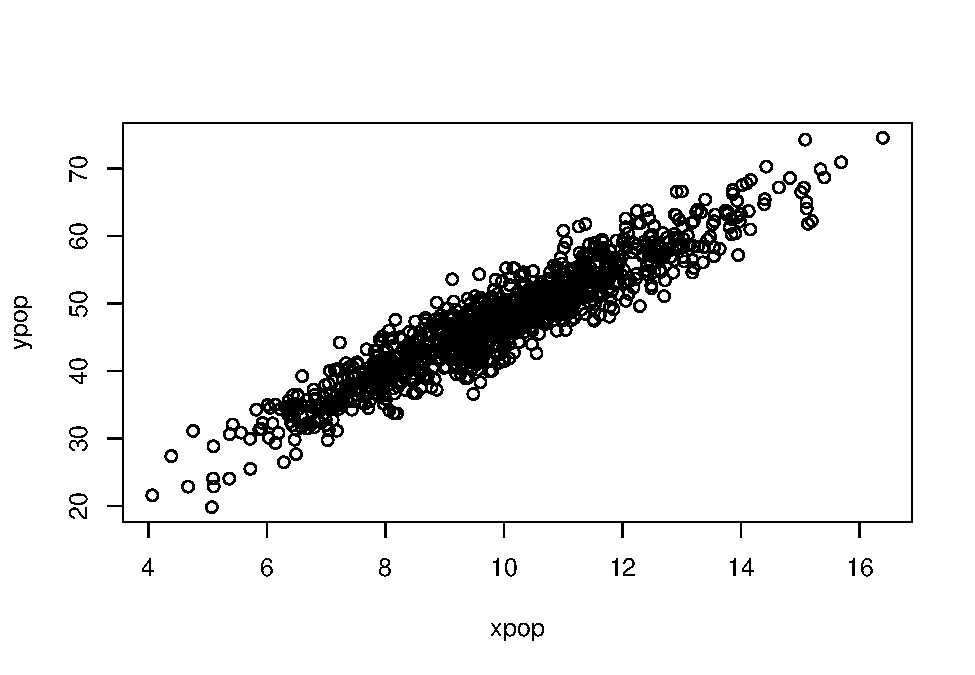
\includegraphics{macroNoGiodP_files/figure-latex/unnamed-chunk-5-1.pdf}

\begin{Shaded}
\begin{Highlighting}[]
\CommentTok{# Check again by running a regression using the lm() function and seeing if the output matches what was calculated }
\KeywordTok{lm}\NormalTok{(ypop }\OperatorTok{~}\StringTok{ }\NormalTok{xpop)}
\end{Highlighting}
\end{Shaded}

\begin{verbatim}
## 
## Call:
## lm(formula = ypop ~ xpop)
## 
## Coefficients:
## (Intercept)         xpop  
##       8.016        3.974
\end{verbatim}

\begin{Shaded}
\begin{Highlighting}[]
\CommentTok{# It does! When we run the regression, the output reports that the intercept is 7.89 and the slope is 4.01 :-) }
\end{Highlighting}
\end{Shaded}

\subsection{Part II}\label{part-ii-2}

\begin{Shaded}
\begin{Highlighting}[]
\CommentTok{# Create a vector which contains the fitted / predicted values; we use the values for beta0hat and beta1hat because this is the estimated line and we must use the values that were generated using our sample data; it is important not to conflate beta0hat and beta1hat with beta 0 and beta 1. }
\NormalTok{yhat <-}\StringTok{ }\KeywordTok{vector}\NormalTok{()}
\NormalTok{residuals <-}\StringTok{ }\KeywordTok{vector}\NormalTok{()}
\ControlFlowTok{for}\NormalTok{ (i }\ControlFlowTok{in} \DecValTok{1}\OperatorTok{:}\DecValTok{1000}\NormalTok{) \{}
\NormalTok{  yhat[i] <-}\StringTok{ }\NormalTok{beta0hat }\OperatorTok{+}\StringTok{ }\NormalTok{beta1hat}\OperatorTok{*}\NormalTok{xpop[i]}
\NormalTok{  residuals[i] <-}\StringTok{ }\NormalTok{ypop[i] }\OperatorTok{-}\StringTok{ }\NormalTok{yhat[i] }
\NormalTok{\}}
\CommentTok{# Self note, do not, when writing loop, assign the output of the DGP to the whole vector because you will only store that one value, you have to remember that you are only storing for one individual "loop" of the process. . .so, here, instead of assigning beta0hat + beta1hat*xpop[i]  to yhat, it should be assigned to yhat[i]}

\CommentTok{# Create a data frame so that all of the values can be compared in a neat, unified way. }
\KeywordTok{tibble}\NormalTok{(}\DataTypeTok{x =}\NormalTok{ xpop, }\DataTypeTok{y =}\NormalTok{ yhat, residuals)}
\end{Highlighting}
\end{Shaded}

\begin{verbatim}
## # A tibble: 1,000 x 3
##        x     y residuals
##    <dbl> <dbl>     <dbl>
##  1 10.0   47.8    -0.907
##  2 12.5   57.6    -1.87 
##  3  9.44  45.5     4.52 
##  4 10.6   50.0    -0.435
##  5 11.3   52.9     1.23 
##  6  8.67  42.5     5.39 
##  7  8.96  43.6    -0.492
##  8 12.9   59.1    -4.51 
##  9  9.06  44.0     2.96 
## 10 12.4   57.3    -2.46 
## # ... with 990 more rows
\end{verbatim}

\begin{Shaded}
\begin{Highlighting}[]
\CommentTok{# Now, I have to actually make the line using these fitted values; plot the fitted values using the historical values for x  }
\KeywordTok{plot}\NormalTok{(xpop, yhat)}
\end{Highlighting}
\end{Shaded}

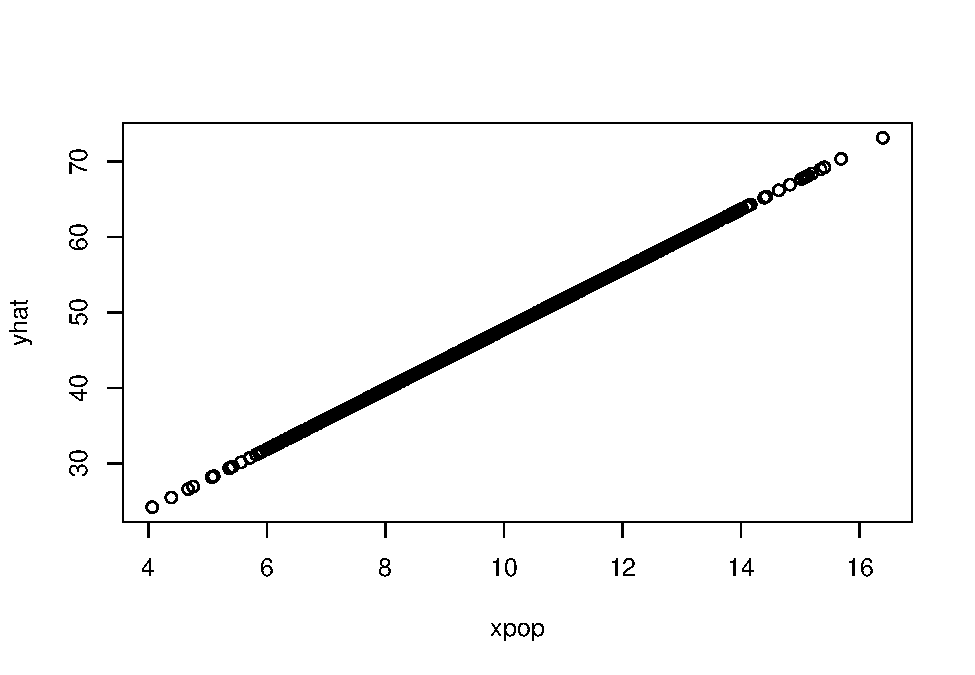
\includegraphics{macroNoGiodP_files/figure-latex/unnamed-chunk-6-1.pdf}

\begin{Shaded}
\begin{Highlighting}[]
\CommentTok{# Now, I will plot the residuals to ensure that they are not heteroskedacic and are, generally, near 0}
\KeywordTok{plot}\NormalTok{(xpop, residuals)}
\end{Highlighting}
\end{Shaded}

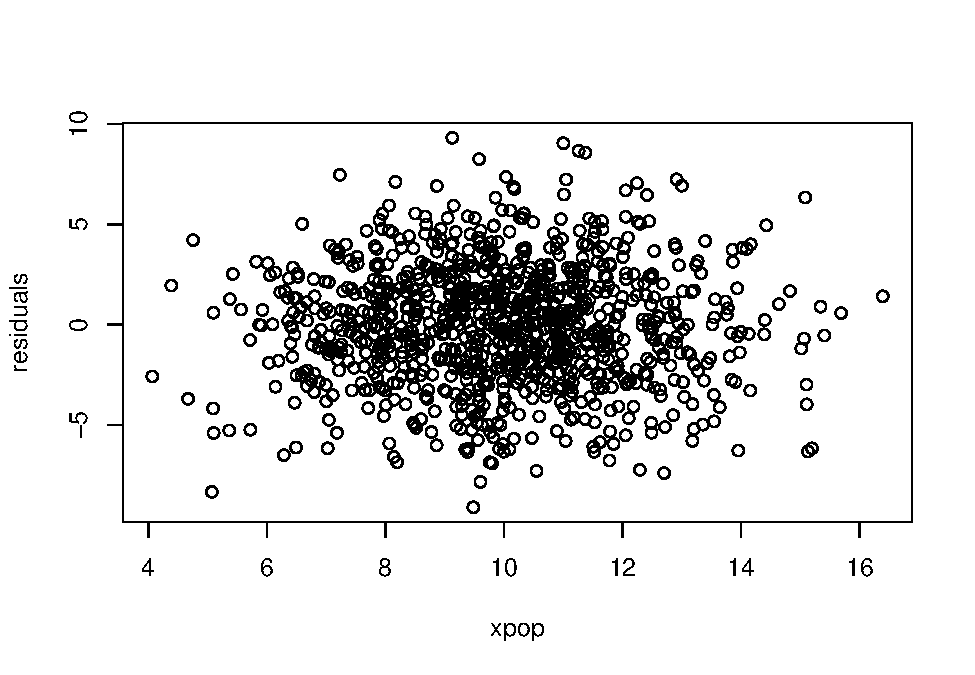
\includegraphics{macroNoGiodP_files/figure-latex/unnamed-chunk-6-2.pdf}

\begin{Shaded}
\begin{Highlighting}[]
\CommentTok{# Yes, these are true. }
\end{Highlighting}
\end{Shaded}

\section{Assignment 4}\label{assignment-4}

\subsection{Part I}\label{part-i-3}

\begin{Shaded}
\begin{Highlighting}[]
\CommentTok{# a. Calculate R squared which is ESS / TSS -- ESS is explained sum of squares which is to say it represents the amount of variation in Y that is explained by X }

\CommentTok{# Calculate ESS components first by writing a loop}
\NormalTok{ESSComp <-}\StringTok{ }\KeywordTok{vector}\NormalTok{()}
\ControlFlowTok{for}\NormalTok{ (i }\ControlFlowTok{in} \DecValTok{1}\OperatorTok{:}\DecValTok{1000}\NormalTok{) \{}
\NormalTok{  ESSComp[i] <-}\StringTok{ }\NormalTok{yhat[i] }\OperatorTok{-}\StringTok{ }\KeywordTok{mean}\NormalTok{(ypop)}
\NormalTok{\}}

\CommentTok{# Then, calculate ESS by summing up the components and squaring}
\NormalTok{ESS <-}\StringTok{ }\KeywordTok{sum}\NormalTok{(ESSComp}\OperatorTok{^}\DecValTok{2}\NormalTok{)}
\NormalTok{ESS}
\end{Highlighting}
\end{Shaded}

\begin{verbatim}
## [1] 62348.8
\end{verbatim}

\begin{Shaded}
\begin{Highlighting}[]
\CommentTok{# ESS is 68158.55 which seems large. . .but could be correct (?)}

\CommentTok{# Find the TSS components which are calculated by using the ypop minus yhat squared}
\NormalTok{TSSComp <-}\StringTok{ }\KeywordTok{vector}\NormalTok{()}
\ControlFlowTok{for}\NormalTok{ (i }\ControlFlowTok{in} \DecValTok{1}\OperatorTok{:}\DecValTok{1000}\NormalTok{) \{}
\NormalTok{  TSSComp[i] <-}\StringTok{ }\NormalTok{ypop[i] }\OperatorTok{-}\StringTok{ }\KeywordTok{mean}\NormalTok{(ypop)}
\NormalTok{\}}

\CommentTok{# Then, calculate TSS by summing up the components and squaring }
\NormalTok{TSS <-}\StringTok{ }\KeywordTok{sum}\NormalTok{(TSSComp}\OperatorTok{^}\DecValTok{2}\NormalTok{)}
\NormalTok{TSS}
\end{Highlighting}
\end{Shaded}

\begin{verbatim}
## [1] 71083.36
\end{verbatim}

\begin{Shaded}
\begin{Highlighting}[]
\CommentTok{# TSS is 76969.14}

\CommentTok{# Now, calculate R squared by dividing ESS by TSS }
\NormalTok{ESS}\OperatorTok{/}\NormalTok{TSS}
\end{Highlighting}
\end{Shaded}

\begin{verbatim}
## [1] 0.8771222
\end{verbatim}

\begin{Shaded}
\begin{Highlighting}[]
\CommentTok{# R squared is 0.89 }

\CommentTok{# b. Show that for any individual observation TSSi ≠ ESSi + RSSi }
\CommentTok{# Calculate the RSS components }
\NormalTok{RSSComp <-}\StringTok{ }\KeywordTok{vector}\NormalTok{()}
\ControlFlowTok{for}\NormalTok{ (i }\ControlFlowTok{in} \DecValTok{1}\OperatorTok{:}\DecValTok{1000}\NormalTok{) \{}
\NormalTok{  RSSComp[i] <-}\StringTok{ }\NormalTok{ypop[i] }\OperatorTok{-}\StringTok{ }\NormalTok{yhat[i]}
\NormalTok{\}}

\CommentTok{# Then, calculate the RSS by summing up the components and squaring }
\NormalTok{RSS <-}\StringTok{ }\KeywordTok{sum}\NormalTok{(RSSComp}\OperatorTok{^}\DecValTok{2}\NormalTok{)}
\NormalTok{RSS}
\end{Highlighting}
\end{Shaded}

\begin{verbatim}
## [1] 8734.565
\end{verbatim}

\begin{Shaded}
\begin{Highlighting}[]
\CommentTok{# RSS is 8810.586}

\NormalTok{babyShark <-}\StringTok{ }\KeywordTok{tibble}\NormalTok{(}\DataTypeTok{ESSi =}\NormalTok{ ESSComp}\OperatorTok{^}\DecValTok{2}\NormalTok{, }\DataTypeTok{RSSi =}\NormalTok{ RSSComp}\OperatorTok{^}\DecValTok{2}\NormalTok{, }\DataTypeTok{TSSi =}\NormalTok{ TSSComp}\OperatorTok{^}\DecValTok{2}\NormalTok{)}
\NormalTok{babySharkMutate <-}\StringTok{ }\NormalTok{dplyr}\OperatorTok{::}\KeywordTok{mutate}\NormalTok{(babyShark, }\DataTypeTok{ERSSi =}\NormalTok{ ESSi }\OperatorTok{+}\StringTok{ }\NormalTok{RSSi)}
\NormalTok{babySharkMutate}
\end{Highlighting}
\end{Shaded}

\begin{verbatim}
## # A tibble: 1,000 x 4
##        ESSi   RSSi    TSSi   ERSSi
##       <dbl>  <dbl>   <dbl>   <dbl>
##  1   0.0372  0.823  0.510    0.860
##  2 100.      3.48  66.3    104.   
##  3   4.28   20.4    5.98    24.7  
##  4   5.71    0.189  3.82     5.90 
##  5  28.8     1.51  43.5     30.3  
##  6  26.0    29.1    0.0871  55.1  
##  7  15.6     0.242 19.7     15.9  
##  8 133.     20.3   49.2    153.   
##  9  12.6     8.75   0.348   21.3  
## 10  93.7     6.03  52.2     99.7  
## # ... with 990 more rows
\end{verbatim}

\begin{Shaded}
\begin{Highlighting}[]
\CommentTok{# You can see on the resulting table that the ERSSi (ESSi + RSSi) ≠ TSSi}

\CommentTok{# Show that this; however, works across all observations }
\NormalTok{babySharkProof <-}\StringTok{ }\KeywordTok{tibble}\NormalTok{(TSS, ESS, RSS)}
\NormalTok{babySharkProofMutate <-}\StringTok{ }\NormalTok{dplyr}\OperatorTok{::}\KeywordTok{mutate}\NormalTok{(babySharkProof, }\DataTypeTok{ERSS =}\NormalTok{ ESS }\OperatorTok{+}\StringTok{ }\NormalTok{RSS)}
\NormalTok{babySharkProofMutate}
\end{Highlighting}
\end{Shaded}

\begin{verbatim}
## # A tibble: 1 x 4
##      TSS    ESS   RSS   ERSS
##    <dbl>  <dbl> <dbl>  <dbl>
## 1 71083. 62349. 8735. 71083.
\end{verbatim}

\begin{Shaded}
\begin{Highlighting}[]
\CommentTok{# In the table, you can see that, across all observations, ERSS (ESS + RSS) = TSS }

\CommentTok{# c. Show that the sum of the residuals is approximately 0}
\KeywordTok{sum}\NormalTok{(residuals)}
\end{Highlighting}
\end{Shaded}

\begin{verbatim}
## [1] 3.186784e-12
\end{verbatim}

\begin{Shaded}
\begin{Highlighting}[]
\CommentTok{# Yes, the output when we sum the residuals is 3.165e-12 which is very, very low and, effectively, approximately 0}

\CommentTok{# Show that sum(x*u) is approximately 0 }
\KeywordTok{sum}\NormalTok{(x}\OperatorTok{*}\NormalTok{residuals)}
\end{Highlighting}
\end{Shaded}

\begin{verbatim}
## [1] 2.530065e-11
\end{verbatim}

\begin{Shaded}
\begin{Highlighting}[]
\CommentTok{# Yes, the output when we sum the x*residuals is 2.855e-11 which is very, very low and, effectively, approximately 0}
\end{Highlighting}
\end{Shaded}

\section{Assignment 5}\label{assignment-5}

\subsection{Part I}\label{part-i-4}

\begin{Shaded}
\begin{Highlighting}[]
\CommentTok{# My coefficient of 4.01 is very close to the true population value of 4; however, it is not exactly the same as the true population value. It may be different because the data generating process is random and we only have one small snapshot or insight into what the larger population might look like. Consequently, while it may be pretty close to being representative of the actual population, it will not be exactly the same because we do not have complete knowledge of the population frame. }
\end{Highlighting}
\end{Shaded}

\subsection{Part II}\label{part-ii-3}

\begin{Shaded}
\begin{Highlighting}[]
\NormalTok{ypop2 <-}\StringTok{ }\KeywordTok{vector}\NormalTok{()}
\NormalTok{x1 <-}\StringTok{ }\KeywordTok{vector}\NormalTok{()}
\NormalTok{x2 <-}\StringTok{ }\KeywordTok{vector}\NormalTok{()}
\ControlFlowTok{for}\NormalTok{ (i }\ControlFlowTok{in} \DecValTok{1}\OperatorTok{:}\DecValTok{1000000}\NormalTok{) \{}
\NormalTok{  x1 =}\StringTok{ }\KeywordTok{rnorm}\NormalTok{(}\DecValTok{1}\NormalTok{, }\DataTypeTok{mean =} \DecValTok{10}\NormalTok{, }\DataTypeTok{sd =} \DecValTok{2}\NormalTok{)}
\NormalTok{  x2 =}\StringTok{ }\KeywordTok{rnorm}\NormalTok{(}\DecValTok{1}\NormalTok{, }\DataTypeTok{mean =} \DecValTok{9}\NormalTok{, }\DataTypeTok{sd =} \DecValTok{2}\NormalTok{)}
\NormalTok{  u =}\StringTok{ }\KeywordTok{rnorm}\NormalTok{(}\DecValTok{1}\NormalTok{, }\DataTypeTok{mean =} \DecValTok{0}\NormalTok{, }\DataTypeTok{sd =} \DecValTok{3}\NormalTok{)}
\NormalTok{  ypop2[i] <-}\StringTok{ }\DecValTok{8} \OperatorTok{+}\StringTok{ }\DecValTok{4}\OperatorTok{*}\NormalTok{x1 }\OperatorTok{+}\StringTok{ }\DecValTok{10}\OperatorTok{*}\NormalTok{x2 }\OperatorTok{+}\StringTok{ }\NormalTok{u }
\NormalTok{  x1[i] <-}\StringTok{ }\NormalTok{x1}
\NormalTok{  x2[i] <-}\StringTok{ }\NormalTok{x2}
\NormalTok{\}}
\end{Highlighting}
\end{Shaded}

\end{document}
